\documentclass[journal]{IEEEtran}
\usepackage[a5paper, margin=10mm]{geometry}
%\usepackage{lmodern} % Ensure lmodern is loaded for pdflatex
\usepackage{tfrupee} % Include tfrupee package


\setlength{\headheight}{1cm} % Set the height of the header box
\setlength{\headsep}{0mm}     % Set the distance between the header box and the top of the text


%\usepackage[a5paper, top=10mm, bottom=10mm, left=10mm, right=10mm]{geometry}

%
\setlength{\intextsep}{10pt} % Space between text and floats

\makeindex


\usepackage{cite}
\usepackage{amsmath,amssymb,amsfonts,amsthm}
\usepackage{algorithmic}
\usepackage{graphicx}
\usepackage{textcomp}
\usepackage{xcolor}
\usepackage{txfonts}
\usepackage{listings}
\usepackage{enumitem}
\usepackage{mathtools}
\usepackage{gensymb}
\usepackage{comment}
\usepackage[breaklinks=true]{hyperref}
\usepackage{tkz-euclide} 
\usepackage{listings}
\usepackage{multicol}
\usepackage{xparse}
\usepackage{gvv}
%\def\inputGnumericTable{}                                 
\usepackage[latin1]{inputenc}                                
\usepackage{color}                                            
\usepackage{array}                                            
\usepackage{longtable}                                       
\usepackage{calc}                                             
\usepackage{multirow}                                         
\usepackage{hhline}                                           
\usepackage{ifthen}                                               
\usepackage{lscape}
\usepackage{tabularx}
\usepackage{array}
\usepackage{float}
\usepackage{ar}
\usepackage[version=4]{mhchem}


\newtheorem{theorem}{Theorem}[section]
\newtheorem{problem}{Problem}
\newtheorem{proposition}{Proposition}[section]
\newtheorem{lemma}{Lemma}[section]
\newtheorem{corollary}[theorem]{Corollary}
\newtheorem{example}{Example}[section]
\newtheorem{definition}[problem]{Definition}
\newcommand{\BEQA}{\begin{eqnarray}}
\newcommand{\EEQA}{\end{eqnarray}}

\theoremstyle{remark}


\begin{document}
\bibliographystyle{IEEEtran}
\onecolumn

\title{1.5.17}
\author{Jnanesh Sathisha Karmar- EE25BTECH11029}
\maketitle


\renewcommand{\thefigure}{\theenumi}
\renewcommand{\thetable}{\theenumi}
\textbf{Question}The midpoint of the line segment joining $\vec{A}\brak{2a, 4}$ and $\vec{B}\brak{-2, 3b}$ is \brak{1, 2a + 1}. Find
the values of a and b.

\textbf{Solution}The midpoint M of line segment AB, with $\vec{A}\brak{x_1, y_1}$ and $\vec{B}\brak{x_2, y_2}$, is:
\begin{align}
	\vec{M}=\frac{\vec{A}+\vec{B}}{2}=\frac{\myvec{x_1\\y_1} + \myvec{x_2\\y_2}}{2}
\end{align}
Given details:
\begin{align}
    \vec{A}=\myvec{2a\\4}  \vec{B}=\myvec{-2\\3b} \vec{M}=\myvec{1\\2a+1}
\end{align}
Substituting the points:
\begin{align}
\frac{\myvec{2a\\4} + \myvec{-2\\3b}}{2}=\myvec{\frac{2a-2}{2}\\ \frac{\brak{4+3b}}{2}}
\end{align}
Equating coordinates, we get two equations:
\begin{align}
\frac{2a - 2}{2} &= 1 \\
\frac{4 + 3b}{2} &= 2a + 1
\end{align}
Using \brak{3} 
\begin{align}
    a=2
\end{align}
Using \brak{3} and \brak{6}
\begin{align}
    b=2
\end{align}
Therefore Values of a and b are both 2
\begin{figure}[H]
    \centering
    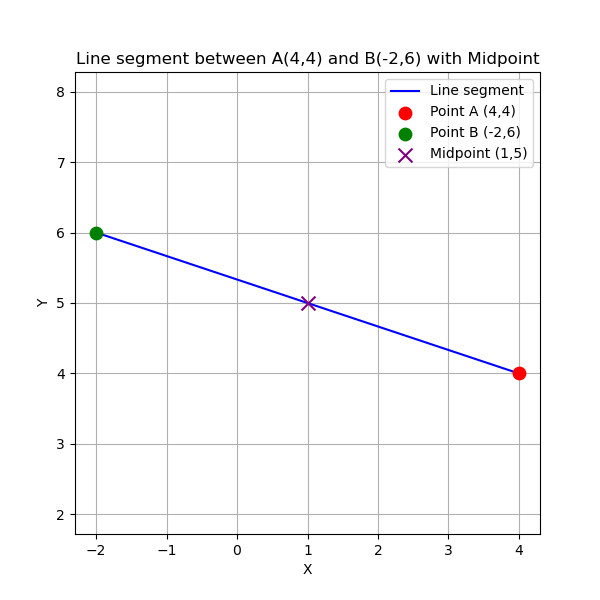
\includegraphics[width=1\linewidth]{figs/line_segment.png}
    \caption{linesegment with 2 points and its midpoint}
    \label{fig:placeholder_1}
\end{figure}
\end{document}